\documentclass[11pt,a4paper]{article}
\usepackage[top=3cm, bottom=2cm, left=2cm, right=2cm]{geometry}
\usepackage[utf8]{inputenc}
% \usepackage[T1]{fontenc}
\usepackage{amsmath, amsfonts, amssymb}
\usepackage{siunitx}
\usepackage[brazil]{babel}
\usepackage{graphicx}
\usepackage[margin=10pt,font={small, it},labelfont=bf, textfont=it]{caption}
\usepackage[dvipsnames, svgnames]{xcolor}
\DeclareCaptionFont{MediumOrchid}{\color[svgnames]{MediumOrchid}}
\usepackage[pdftex]{hyperref}
\usepackage{natbib}
\bibliographystyle{plainnat}
\bibpunct{[}{]}{,}{s}{}{}
\usepackage{color}
\usepackage{footnote}
\usepackage{setspace}
\usepackage{booktabs}
\usepackage{multirow}
\usepackage{subfigure}
\usepackage{fancyhdr}
\usepackage{leading}
\usepackage{indentfirst}
\usepackage{wrapfig}
\usepackage{mdframed}
\usepackage{etoolbox}
\usepackage[version=4]{mhchem}
\usepackage{enumitem}
\usepackage{caption}
\usepackage{titlesec}
\usepackage{tcolorbox}
\usepackage{tikz}
\usepackage{LobsterTwo}
\usepackage[T1]{fontenc}
\usepackage{fontspec}
\usepackage{txfonts}
\AtBeginEnvironment{equation}{\fontsize{13}{16}\selectfont}


\titleformat{\section}{\LobsterTwo\LARGE\color{CarnationPink}}{\thesection.}{1em}{}
\titleformat{\subsection}{\LobsterTwo\LARGE\color{CarnationPink}}{\thesubsection}{1em}{}


\DeclareCaptionLabelFormat{figuras}{\textcolor{DarkTurquoise}{Figura \arabic{figure}}}
\captionsetup[figure]{labelformat=figuras}

\makeatletter
\renewcommand\tagform@[1]{\maketag@@@{\color{CarnationPink}(#1)}}
\makeatother

\renewcommand{\theequation}{Eq. \arabic{equation}}
\renewcommand{\thefigure}{Fig. \arabic{figure}}
\renewcommand{\thesection}{\textcolor{CarnationPink}{\arabic{section}}}

\setlist[itemize]{label=\textcolor{CarnationPink}{$\mathbf{\square}$}}

\setlist[enumerate]{label=\textcolor{CarnationPink}{\arabic*.}, align=left}


\newcounter{exemplo}

\NewDocumentEnvironment{exemplo}{ O{} }{%
\allowbreak
\setlength{\parindent}{0pt}
  \begin{mdframed}[
  leftline=true,
  topline=false,
  rightline=false,
  bottomline=false,
  linewidth=2pt,
  linecolor=CarnationPink,
  frametitlerule=false,
  frametitlefont=\LobsterTwo\large\color{CarnationPink},
  frametitle={\color{CarnationPink}\LobsterTwo\large #1},
  ]
}{%
  \end{mdframed}
}

\setlength{\fboxsep}{5pt}
\setlength{\fboxrule}{1.5pt}
\usepackage{float}
\renewcommand{\thefootnote}{\alph{footnote}}
\usepackage{url}
\hypersetup{
	colorlinks=true,
	linkcolor=DarkTurquoise,
	filecolor=DarkTurquoise,      
	urlcolor=DarkTurquoise,
	citecolor=DarkTurquoise,
	pdftitle={Radioterapia}
}
\pagestyle{fancy}
\fancyhf{}
\renewcommand{\headrulewidth}{0pt}
\rfoot{Página \thepage}

\title{\LobsterTwo\Huge{Radioterapia}}
\author{\LobsterTwo{Parâmetros e Cálculos De Unidades Monitoras}\nocite{*}}
\date{\LobsterTwo\textit{Dalila Mendonça}}
\begin{document}
	\maketitle

    \section{Parâmetros de Cálculo de Dose}

    A dose em um ponto no meio é composta por duas componentes: \textit{\textcolor{MediumOrchid}{Componente Primária e componente de espalhamento}}. A componente de dose primária é devido ao feixe primário, ou seja, aos fótons originais produzidos, enquanto que a componente de  dose espalhada é devido aos fótons do feixe primário que foram espalhados após interagir e transferir energia para a partícula carregada do meio.

    A dose espalhada pode ser subdividida em outras duas componentes, uma vez que essas componentes podem variar independente uma da outra: \textit{\textcolor{MediumOrchid}{Componente devido ao espalhamento no colimador e componente devido ao espalhamento no phantom}}; Por exemplo, bloquear uma parte do campo não fará com que tenha uma mudança significativa na fluência de energia dos fótons que saem pela parte aberta do campo, porém irá mudar significativamente (reduzir) o espalhamento no meio dependendo ta extensão da região bloqueada.

    Uma forma de determinar as componentes devido ao espalhamento é considerando que o espalhamento pelo colimador é parte do feixe primário, permitindo que o espalhamento no phantom seja calculado separadamente. Deste modo, a dose primária efetiva é a dose devido ao feixe primário e ao feixe espalhado pelo colimador, e, portanto, a dose primária efetiva no phantom é a dose total menos a dose espalhada no phantom. Alternativamente, a dose primária efetiva pode ser definida como a dose esperada em um campo quando o volume de espalhamento é reduzido à zero enquanto a abertura do colimador se mantém constante, ou seja, é a dose para o determinado tamanho de campo onde nenhum fótons espalhado alcance esse ponto. 

    Uma vez que ocorre a perda de equilíbrio lateral em campos muito estreitos (campos 0 x 0), a medida direta do feixe primário é praticamente impossível. Uma possibilidade seria através de sistemas que simulam o transporte de elétrons no cálculo das componentes primária e espalhada, porém ainda não estão totalmente desenvolvidos e implementados para a rotina. 

    Portanto, supõe-se que exista um campo 0 x 0 de modo que haja equilíbrio lateral em todos os pontos. Esse campo é obtido através da extrapolação da curva da dose na profundidade em função do tamanho de campo. Normalmente utiliza-se o menor campo possível, porém grande o suficiente para fornecer o equilíbrio eletrônico lateral (normalmente os campos \qtyproduct{3 x 3}{cm} ou \qtyproduct{4 x 4}{cm}) e então a curva é extrapolada para o campo \qtyproduct{0 x 0 }{cm}.

    \section{Fator de Espalhamento do Colimador (Razão do Output no Ar)}
\
    O output do feixe (taxa de exposição, taxa de dose no ar ou taxa de fluência de energia) medido no ar depende do tamanho de campo. A medida que o tamanho de campo aumenta, o output aumenta devido ao aumento do espalhamento no colimador que é adicionado ao feixe primário.

    O \textit{\textcolor{MediumOrchid}{fator de espalhamento do colimador $(S_c)$}} é definido como a razão entre o output no ar para um dado tamanho de campo e o output no ar para o campo de referência, normalmente definido como o campo \qtyproduct{10 x 10}{cm}. O $S_c$ pode ser medido com uma câmara de ionização com uma capa de buildup larga o suficiente para fornecer o buildup de dose máximo para a energia do feixe em questão. 
    
    \begin{figure}[h]
        \centering
        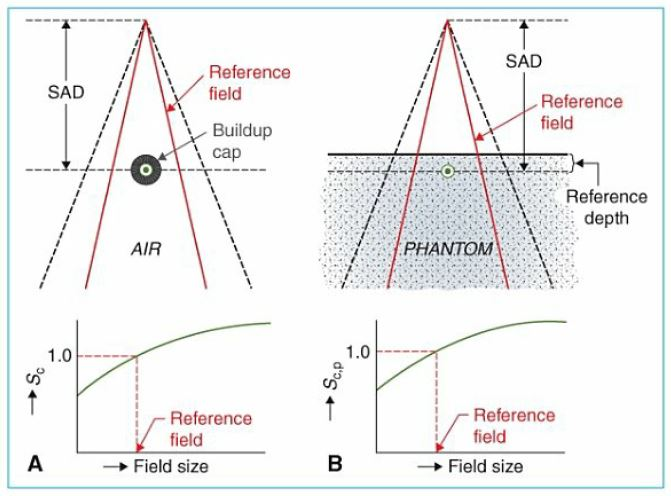
\includegraphics[width=0.8\textwidth]{Imagens/scEScp.JPG}
        \caption{Setup para obtenção do $S_c$ e $S_{c,p}$}
        \label{fig:scEScp}                
    \end{figure}

    A \ref{fig:scEScp}\textcolor{DarkTurquoise}{(A)} mostra o setup de medidas para obter o fator $S_c$; As medidas feitas com a câmara de ionização são plotadas em função do tamanho de campo (ou através do lado do quadrado equivalente ou através da razão A/P) e então os valores são normalizados pela medida do campo de referência \qtyproduct{10 x 10}{cm}. 

    \begin{wrapfigure}{l}{0.25\textwidth}
        \centering
        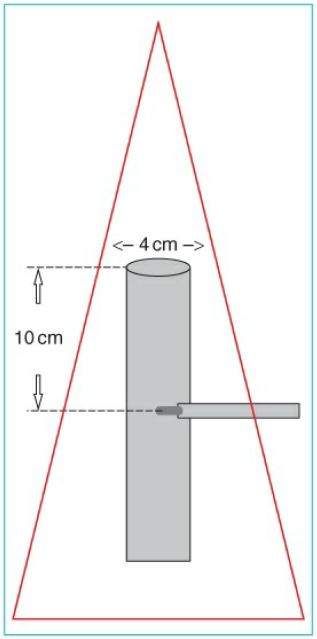
\includegraphics[width=0.2\textwidth]{Imagens/miniphantom.JPG}
        \caption{Miniphantom para medida do $S_c$} 
        \label{fig:miniphantom}
    \end{wrapfigure}

    Na medida do $S_c$, o campo deve cobrir completamente a capa de buildup de modo que a capa não fique sob regiões de penumbra (bordas dos campos) em todos os tamanhos de campos caso as medidas tenham que refletir a fluência relativa de energia dos fótons. É necessário uma margem entre a borda do campo e a capa de buildup de no mínimo 1 cm.
    
    A capa de buildup necessária para feixes de megavoltagem é muito larga de modo que seja impraticável a medida do $S_c$. Para estes casos, foi proposto a utilização de um miniphantom, apresentado na \ref{fig:miniphantom}, que se trata de um phantom coaxial cilíndrico estreito (4 cm de diâmetro) com uma profundidade para medição além de $d_{max}$  de 10 cm, sendo o suficiente  para evitar a contaminação de elétrons presente no feixe primário.

    Normalmente os fatores $S_c$ para os campos são medidos com a câmara de ionização posicionada na SAD. Porém, para campos pequenos, pode-se realizar as medidas de output (tanto para o campo em análise como para o campo de referência) em distâncias maiores que a SAD de modo que o menor campo cubra o limite da capa de buildup ou o miniphantom com uma margem adequada, porém o tamanho de campo segue sendo definido na SAD (e não na projeção na distância além da SAD).

    \section{Fator de Espalhamento no Phantom}

    O \textit{\textcolor{MediumOrchid}{fator de espalhamento no phantom $S_p$}} considera as mudanças na radiação espalhada na profundidade de referência devido ao espalhamento originado no phantom a medida que o tamanho de campo é alterado. O fator $S_p$ pode ser definido como a razão entre a taxa de dose (ou dose por MU) para um dado tamanho de campo (aberto pelos colimadores secundários) na profundidade de referência e a taxa de dose no mesmo ponto para um tamanho de campo de referência \qtyproduct{10 x 10}{cm} (campo colimado pelos colimadores terciários como MLC, blocos de cerrobend, etc\dots) mantendo a mesma abertura de colimador (ou seja, a mesma fluência de energia incidente). Portanto, o fator $S_p$ está relacionado à mudanças de volume de phantom irradiado para uma abertura fixa de colimador, ou seja, ao abrir um campo com os jaws, um determinado volume será irradiado, e mantendo essa abertura dos jaws, um campo colimado de referência irá irradiar um volume diferente.  Portanto, o $S_p$ pode ser determinado utilizando o maior tamanho de campo possível e utilizar vários phantoms com diferentes tamanhos de seção transversal. 


    Para feixes de fótons com energia até o \ce{^{60}Co} onde o BSF pode ser determinado precisamente, o $S_p$ na profundidade de dose máxima pode ser definido simplesmente pela razão do BSF para um dado tamanho de campo e o BSF para o campo de referência, ou seja:

        \begin{equation}
            S_p(r) = \frac{BSF(r)}{BSF(r_0)}
            \label{eq:spBsf}
        \end{equation}

    \begin{exemplo}[onde:]
        \begin{itemize}
            \item \textcolor{MediumOrchid}{$r$} é o lado do campo quadrado equivalente; e
            \item \textcolor{MediumOrchid}{$r_0$} é o lado do campo de referência.
        \end{itemize}
    \end{exemplo}

    Uma forma de obter o $S_p$ para qualquer energia é determinando o $S_p$ indiretamente através da equação:

        \begin{equation}
            S_{p}(r) = \frac{S_{c,p}(r)}{S_c(r)}
            \label{eq:scpPraSp}
        \end{equation}

        \begin{exemplo}[onde:]
            \begin{itemize}
                \item \textcolor{MediumOrchid}{$S_{c,p}(r)$} é o fator de espalhamento total definido como a taxa de dose (ou dose por MU) na profundidade de referência para um dado tamanho de campo $r$ dividida pela taxa de dose no mesmo ponto e profundidade para o campo de referência (\ref{fig:scEScp} \textcolor{DarkTurquoise}{(B)}).
            \end{itemize}
        \end{exemplo}

    Desse modo, o fator $S_{c,p}$ contém tanto o fator de espalhamento do colimador quanto o fator de espalhamento no phantom.

    \section{Razão Tecido-Phantom e Razão Tecido-Máximo}

    A TPR é definida como a razão entre a taxa de dose em uma dada profundidade no phantom e a taxa de dose na mesma distância fonte ao ponto (SPD) mas na profundidade de referência. A \ref{fig:tprTmr} ilustra o setup de como a TPR é obtida. A quantidade correspondente para os cálculos de dose espalhada é chamada de Razão Espalhamento-phantom (SPR). 

    \begin{figure}[h]
        \centering
        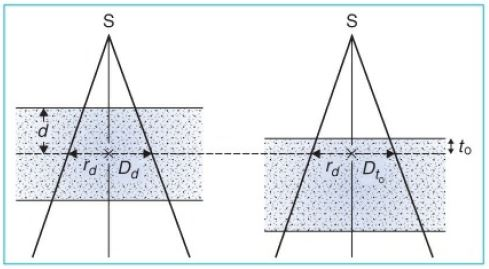
\includegraphics[width=0.8\textwidth]{Imagens/tprTmr.JPG}
        \caption{Definição de TPR e TMR}
        \label{fig:tprTmr}                
    \end{figure}

    A TRP pode ser normalizada em qualquer profundidade de referência (como a utilizada na dosimetria, definida a 10 cm), porém para fins de simplicidade e convenções a profundidade de referência costuma ser definida na profundidade de dose máxima $d_{max}$; Neste caso, a TPR se torna a TMR, ou seja, a TMR é um caso especial da TPR, de modo que é definida como a razão entre a taxa de dose para um dado ponto no phantom e a dose na mesma distância do ponto à fonte, definido na profundidade de dose máxima (\ref{fig:tprTmr}). 
    
    A profundidade de dose máxima em feixes de megavoltagem varia com o tamanho de campo e com a SSD devido ao aumento da contaminação do feixe primário com elétrons que incidem na superfície do phantom/paciente. Portanto, para os cálculos serem independentes da contaminação com elétrons, a profundidade de referência utilizada para a normalização não pode ser definida na região de buildup, ou seja, a profundidade de referência deve ser maior que o alcance dos elétrons. 

    Quanto maior o tamanho de campo e quanto menor a SSD, maior será a contaminação com elétrons; E portanto, $d_{max}$ tende a diminuir (se aproximar da superfície) a medida que o tamanho de campo aumenta e $d_{max}$ tende a aumentar (se afastar da superfície) a medida que a SSD aumenta. Portanto se $d_{max}$ for escolhida para ser a profundidade de referência, então $d_{max}$ deve ser definida para o menor tamanho de campo possível que ainda garanta equilíbrio eletrônico lateral (\qtyproduct{3 x 3}{cm}) e para a maior SSD possível (100 cm ou maior) para obter $d_{max}$ em uma configuração que minimiza os efeitos da contaminação com elétrons na determinação da profundidade de dose máxima. Outra forma de se obter $d_{max}$ é plotando uma curva da $\%DD \times (SSD + d)^2$ em função da profundidade $d$ para encontrar $d_{max}$. Esta relação elimina a dependência de $d_{max}$ com a SSD de modo que $d_{max}$ pode ser obtido plotando $d_{max}$ em função do tamanho de campo ( diminuindo o tamanho de campo até o campo  \qtyproduct{3 x 3}{cm}) e então extrapolando para o campo \qtyproduct{0 x 0}{cm}.

    A profundidade de referência $d_{max}$ deve se manter a mesma para todos os tamanhos de campo e todas as quantidades dosimétricas relevantes como a PDP, TMR, Sp e o fator de calibração do acelerador devem ser normalizados na profundidade $d_{max}$. 


    \begin{tcolorbox}[width=\textwidth, colback={white}, colbacktitle={DarkTurquoise!50!white}, title={$\bigstar$ \LobsterTwo{Observação} $\bigstar $}, coltitle={CarnationPink}, colframe={DarkTurquoise}, fonttitle=\rmfamily\bfseries\Large]
        Deve-se atentar à profundidade de referência $d_0$ utilizada na definição dos fatores. Por exemplo, se os cálculos de dose forem baseados na TPR e na determinação da TPR for escolhido $d_0 = 10 \; cm$, todos os outros parâmetros dosimétricos relevantes, incluindo o fator de calibração do acelerador, deverão ser normalizados na mesma profundidade $d_0 = 10\; cm$;
    \end{tcolorbox}

    O TG-71 consiste em um protocolo para cálculo de MU, e estabelece que qualquer profundidade de referência para normalização será aceitável desde que esta profundidade seja invariante com o tamanho de campo e seja $\geq d_{max}$. Para evitar erros nas conversões, o TG-71 recomenda escolher uma profundidade de normalização fixa na profundidade de 10 cm para efetuar os cálculos de dose de todas as energias de fótons.

    \subsection{Relação entre a PDP e a TMR}

    Para os valores de TMR, assume-se que a fração da contribuição de espalhamento para a dose na profundidade em um determinado ponto é independente da divergência do feixe, dependendo apenas da profundidade do ponto (com respeito à superfície) e o tamanho de campo projetado nessa profundidade. A \ref{fig:tmrECampo} mostra o comportamento de uma curva TMR com a profundidade para diferentes tamanhos de campos para um feixe de 10 MV. 

    \begin{figure}[h]
        \centering
        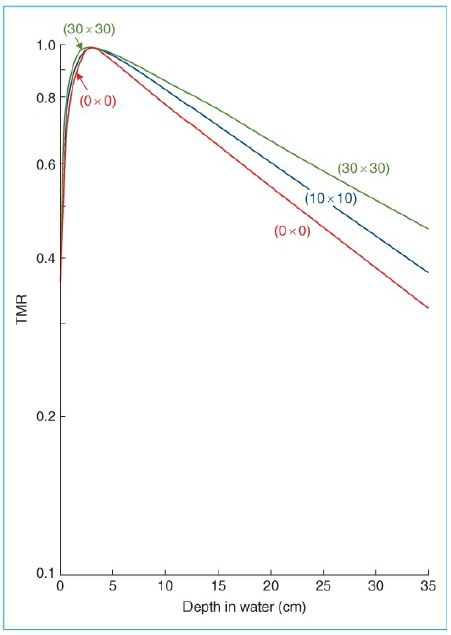
\includegraphics[width=0.4\textwidth]{Imagens/tmrECampo.JPG}
        \caption{TMR em função da profundidade para diferentes tamanhos de campo com um feixe de 10 MV}
        \label{fig:tmrECampo}                
    \end{figure}
    
    A extrapolação para o campo 0 x 0 mostra uma queda mais acentuada com a profundidade quando comparado com os demais tamanhos de campo; Isto se deve unicamente devido a atenuação do feixe primário, que pode ser aproximadamente dado por:

        \begin{equation}
            TMR(d, 0) = e^{-\mu_{eff}(d - d_{max})}
        \end{equation}

    \begin{exemplo}[onde:]
        \begin{itemize}
            \item \textcolor{MediumOrchid}{$\mu_{eff}$} é o coeficiente de atenuação efetivo; O $\mathbf{\mu_{eff}}$ pode ser determinado a partir dos dados da TMR plotando $\mathbf{\mu_{eff}}$ como função do tamanho de campo e extrapolando para o campo 0 x 0. 
        \end{itemize}
    \end{exemplo}

    A TMR e a PDP estão relacionadas a partir da seguinte equação:

        \begin{equation}
            TMR(d, r_d) = \left(\frac{P(d, r, f)}{100}\right)\left(\frac{f + d}{f + d_{max}}\right)^2 \left(\frac{S_p(r_{d_{max}})}{S_p(r_{d})}\right)
            \label{eq:tmrParaPDP}
        \end{equation}

        \begin{exemplo}[onde:]
            \begin{itemize}
                \item \textcolor{MediumOrchid}{$P$} é a PDP na profundidade de interesse; A PDP é normalizada em $d_{max}$ de modo que a $PDP(d_{max}, r, f) = 100$ para todos os tamanhos de campo e para todas as SSDs;
                \item \textcolor{MediumOrchid}{$d$} é a profundidade onde deseja-se avaliar a dose;
                \item \textcolor{MediumOrchid}{$d_{max}$} é a profundidade de referência estabelecida em $d_{max}$; 
                \item \textcolor{MediumOrchid}{$r$} é o tamanho de campo na superfície;
                \item \textcolor{MediumOrchid}{$f$} é a SSD;
                \item \textcolor{MediumOrchid}{$r_d$} $= r \left(\frac{f + d}{f}\right)$
                \item \textcolor{MediumOrchid}{$r_{d_{max}}$} = $r\left(\frac{f + d_{max}}{f}\right)$
            \end{itemize}
        \end{exemplo}

    Portanto, embora a TMR possa ser medida diretamente, ela também pode ser determinada a partir da PDP através da \ref{eq:tmrParaPDP}. Para determinar a TMR do \ce{^{60}Co}, pode-se utilizar a \ref{eq:scpPraSp}  e a \ref{eq:tmrParaPDP}. Além disso, é possível obter a TMR a partir dos dados da TAR para os casos fornecido para os casos como o \ce{^{60}Co} onde a TAR é precisamente definida e conhecida, através da relação:

        \begin{equation}
            TMR(d,r_d) = \left(\frac{TAR(d, r_d)}{TAR(d_{max}, r_d)}\right) = \frac{TAR(d,r_d)}{BSF(r_d)}
            \label{eq:tmrTar}
        \end{equation}

    \subsection{Relação Entre a TPR e a PDP}

    A \ref{eq:tmrParaPDP} pode ser generalizada para a TPR em uma profundidade de referência (por exemplo \qty{10}{cm}):

        \begin{equation}
            TPR(d, r_d) =  \left(\frac{P_N(d, r, f)}{100}\right) \left(\frac{f + d}{f + d_0}\right)^2 \left(\frac{S_p(r_{d_0})}{S_p(r_d)}\right)
        \end{equation}

    \begin{exemplo}[onde:]
        \begin{itemize}
            \item \textcolor{MediumOrchid}{$d_0$} é a profundidade de referência;
            \item \textcolor{MediumOrchid}{$P_N$} é a PDP normalizada na profundidade de referência que pode ser obtida através da PDP regular através da equação: 
            $$P_N(d, r, f) = \frac{P(d, r, f)}{P(d_0, r, f)}$$
            \item \textcolor{MediumOrchid}{$r_{d_0}$} $= r\left(\frac{f + d_0}{f}\right)$
        \end{itemize}
    \end{exemplo}

    \subsection{SPR e SMR}

    A SPR e a SMR são grandezas definidas especialmente para os cálculos da dose espalha no meio, De modo que a SPR e a SMR estão relacionadas com a TPR e a TMR da mesma forma que a SAR está relacionada com a TAR.  Matematicamente, essas quantidades são definidas como:

        \begin{equation}
            SMR(d, r_d) = TMR(d, r_d) \left(\frac{S_p(r_d)}{S_p(0)}\right) - TMR(d,0)
            \label{eq:smrTmr}
        \end{equation}

    e,

        \begin{equation}
            SPR (d,r_d) = TPR(d,r_d) \left(\frac{S_p(r_d)}{S_p(0)}\right) - TPR(d,0)
            \label{eq:sprTpr}
        \end{equation}

        A partir das \ref{eq:spBsf}, \ref{eq:tmrTar} e \ref{eq:smrTmr} pode-se mostrar que os valores de SMR para um feixe de \ce{^{60}Co} são aproximadamente os mesmos valores para a SAR. No entanto, para altas energias, os valores de SMR  podem ser determinados a partir da TMR através da \ref{eq:smrTmr}.

        Como a TMR é normalizada na profundidade de dose máxima, por definição, se modo que seu valor em $d_{max}$ é igual a 1, ou seja $TMR(d_{max}, r_{d_{max}}) = 1$ podemos simplificar a \ref{eq:smrTmr} de modo que:

            Fazendo $\Rightarrow d = d_0 = d_{max}$, temos:

            $$
                SMR(d_{max}, r_{d_{max}}) = TMR(d_{max}, r_{d_{max}}) \left(\frac{S_p(r_d)}{S_p(0)}\right) - TMR(d_{max},0)
            $$    
            \begin{equation}
                SMR(d_{max}, r_{d_{max}}) = \left(\frac{S_p(r_{d_{max}})}{S_p(0)}\right) - 1
                \label{eq:smrSp}
            \end{equation}

        Semelhantemente para a TPR, que é normalizada na profundidade de referência assumindo o valor de uma unidade nessa profundidade, ou seja $TPR(d_0,r_{d_0}) = 1$, temos então:

        \begin{equation}
            SPR(d_{0}, r_{d_{0}}) = \left(\frac{S_p(r_{d_0})}{S_p(0)}\right) - 1
            \label{eq:sprSp}
        \end{equation}



    \section{Formalismo Para o Cálculo de MU}

        O formalismo para cálculo do número de MU irá depender da técnica utilizada no setup de planejamento, onde algumas instituições optam exclusivamente pela técnica isocentrica (SAD), enquanto outros utilizam técnicas da SAD e SSD.

    \subsection{Equações Para o Cálculo de MU}

    Técnica Isocêntrica
        \begin{equation}
            MU = \frac{D}{D_{cal} \cdot S_c(r_c) \cdot S_p(r_d) \cdot TPR(d, r_d) \cdot 
            WF(d, r_d, x) \cdot TF \cdot OAR(d, x) \left(\frac{SCD}{SPD}\right)^2}
            \label{eq:muTpr}
        \end{equation}
    Ou,
        \begin{equation}
            MU = \frac{D}{D_{cal} \cdot S_c(r_c) \cdot S_p(r_d) \cdot TPR(d, r_d) \cdot 
            WF(d, r_d, x) \cdot TF \cdot OAR(d, x) \left(\frac{SCD}{SPD}\right)^2}
            \label{eq:muTmr}
        \end{equation}  

    

    Técnica Não Isocêntrica
        \begin{equation}
            MU = \frac{D}{D_{cal} \cdot S_c(r_c) \cdot S_p(r) \cdot \frac{PDP(d, r, f)}{100} \cdot WF(d, r_d, x) \cdot TF \cdot OAR(d, x) \left(\frac{SCD}{f + d_{max}}\right)^2}
            \label{eq:mupdpdmax}
        \end{equation}  
    Ou,
        \begin{equation}
            MU = \frac{D}{D_{cal} \cdot S_c(r_c) \cdot S_p(r) \cdot \frac{PDP_N(d, r, f)}{100} \cdot WF(d, r_d, x) \cdot TF \cdot OAR(d, x) \left(\frac{SCD}{f + d_{0}}\right)^2}
            \label{eq:mupdpdref}
        \end{equation}  
    

    \begin{exemplo}[onde:]
        \begin{itemize}
            \item \textcolor{MediumOrchid}{$r_c$} é o tamanho de campo definido pelo colimador;
            \item \textcolor{MediumOrchid}{$r_d$} é o tamanho de campo projetado na profundidade d;
            \item \textcolor{MediumOrchid}{$r$} é o tamanho de campo na superfície;
            \item \textcolor{MediumOrchid}{$x$} é a distância off-axis (distância radial do pont de análise ao eixo)
            \item \textcolor{MediumOrchid}{$f$} é a SSD;
            \item \textcolor{MediumOrchid}{$D$} é a dose a ser entregue no ponto de interesse;
            \item \textcolor{MediumOrchid}{$D_{cal}$} é o fator de calibração dado em dose por MU na profundidade de referência ($d_{ref}$) sob as condições de referência;
            \item \textcolor{MediumOrchid}{$S_c(r_c)$} é o fator de espalhamento do colimador definido para um tamanho de campo de colimador $r_c$
            \item \textcolor{MediumOrchid}{$S_p(r)$} é o fator de espalhamento do phantom na $d_{ref}$ para um tamanho de campo $r$ na superfície;
            \item \textcolor{MediumOrchid}{$S_p(r_d)$} é o fator de espalhamento do phantom na $d_{ref}$ para um tamanho de campo $r_d$ na profundidade $d$;
            \item \textcolor{MediumOrchid}{$PDP(d, r, f)$} é a PDP  na profundidade $d$ quando $d_{ref}$ é determinado em $d_{max}$;
            \item \textcolor{MediumOrchid}{$PDP_N(d, r, f)$} é a PDP na profundidade $d$ normalizada para uma profundidade de referência $d_{0}$ diferente de $d_{max}$;
            \item \textcolor{MediumOrchid}{$WF(d, r_d, x)$} é o fator filtro na profundidade $d$ para um tamanho de campo na profundidade $r_d$ e em uma distância off-axis x;
            \item \textcolor{MediumOrchid}{$OAR(d, x)$} é o fator off-axis na profundidade $d$ em uma distância $x$ do eixo central.
            \item \textcolor{MediumOrchid}{$TF$} é o fator bandeja;
            \item \textcolor{MediumOrchid}{$SCD$} é a distância da fonte até ao ponto de calibração onde foi especificado $D_{cal}$;
            \item \textcolor{MediumOrchid}{$SPD$} é a distância da fonte até ao ponto de interesse, onde deseja-se entregar a dose;
            \item \textcolor{MediumOrchid}{$d_{0}$} é a profundidade de referência para a $TPR$ e a $PDP_N$;
            \item \textcolor{MediumOrchid}{$d_{max}$} é a profundidade de dose máxima utilizada para a $PDP$ e a $TMR$;
        \end{itemize}
    \end{exemplo}

    Nas equações para o cálculo das MUs, assume-se que:

    \begin{itemize}[label=\textcolor{CarnationPink}{$\star$}]
        \item O fator de calibração por MU $D_{cal}$ é determinado para a distância do ponto de calibração à fonte, para o tamanho de campo de referência, na profundidade de referência.
        \item A $d_{ref}$ tanto para a determinação de $D_{cal}$ tanto para o $S_p$ deve ser a mesma que  a $d_{ref}$ definida para a quantidade dosimétrica com o qual esses fatores serão utilizados juntamente para a determinação das MUs.
        \item O Fator bandeja (TF) é um fator de transmissão para a bandeja utilizada para fixar os blocos dentre outros acessórios, independente do tamanho de campo e da profundidade de interesse;
        \item A IDQ é válida para a mudança na fluência da energia do fóton no ar em função da distância da fonte. 
    \end{itemize}


    \begin{tcolorbox}[width=\textwidth, colback={white}, title={$\bigstar$ \LobsterTwo{Observação} $\bigstar $}, coltitle={CarnationPink}, colframe={DarkTurquoise}, fonttitle=\rmfamily\bfseries\Large]

        Embora exista um fator no cálculo da MU relacionado ao Inverso do quadrado da distância, tanto para a técnica isocêntrica quanto para técnica não isocêntrica, este fator é inserido para corrigir o fator de calibração nos casos em que a profundidade de referência utilizada para determinar o fator é diferente daquela utilizada nos demais parâmetros. Essa alteração se baseia apenas no IQD devido o fator de calibração ser definido em $d_{max}$ e como citado anteriormente, a fluência de energia no ar varia de acordo com a IQD. Outros parâmetros, no entanto, podem não ter uma correção apenas devido à IDQ, devido ao fator ser determinado para uma profundidade no tecido de forma que somente a IQD não irá fornecer a variação da fluência de fótons, sendo necessário considerar a atenuação e o espalhamento. 
    \end{tcolorbox}

    \subsection{Cálculo Para as Unidades de \ce{^{60}Co}}

        Os métodos já fornecidos são gerais de modo que também podem ser aplicados ao \ce{^{60}Co}. A diferença é que os feixes de \ce{^{60}Co} normalmente são calibrados em termos da taxa de dose no ar ou em termos da taxa de dose no phantom de modo que deve-se determinar o tempo de tratamento para entregar a dose total. Desse modo, deverão ser obtidos os seguintes parâmetros:

        \begin{enumerate}[label=\textcolor{CarnationPink}{(\alph*)}]
            \item A taxa de Dose no Phantom $D_0(t_0, r_0, f_0)$ na profundidade de dose máxima $d_0$, par ao tamanho de campo de referência $r_0$ para a SSD padrão $f_0$;
            \item O fator $S_c$;
            \item O fator $S_p$;
            \item Os valores de $PDP$;
            \item Os valores de $TMR$
        \end{enumerate}

        Se foram adquiridos os dados de PDP, o $S_p$ poderá ser determinado através da \ref{eq:spBsf} e a $TMR$ poderá ser obtida através da \ref{eq:tmrTar}.


    \section{Campos Irregulares}

        A análise dosimétrica para campos irregulares utilizando a TMR e SMR ou a TPR e SPR é análoga ao método utilizado através da TAR e SAR.  Para um campo irregular utilizando o método da integral de Clarkson, onde um campo irregular em uma profundidade $d$ é dividido em n setores, então será determinada a média da SPR ou TPR através dos dados obtidos e então determinar a dose no isocentro.

        $$\overline{SPR}(d, r_d) = \frac{1}{n} \sum_{i = 2}^{n} SPR(d, r_i)$$


        onde $r_i$ é o raio do i-ésimo setor na profundidade d e n é o número total de setores $(n = 2\pi/\Delta \theta)$ onde $\Delta\theta$  é o ângulo de setor;

        O valor determinado para $\overline{SPR}(d, r_d)$ é então convertido para o $\overline{SPR}(d, r_d)$ utilizando a \ref{eq:sprTpr}:


        $$\overline{TPR}(d, r_d) = \left[TPR(d,0) +\overline{SPR}(f, r_d)\right]\times \frac{S_p(0)}{\bar{S}_p(r_d)}$$

        \begin{exemplo}[onde]
            \begin{itemize}
                \item \textcolor{MediumOrchid}{$\bar{S}_p(r_d)$} é o fator médio de espalhamento do phantom para um campo irregular; e
                \item \textcolor{MediumOrchid}{$S_p(0)$} é o fator de espalhamento do phantom para o campo 0 x 0;
            \end{itemize}
        \end{exemplo}

        A equação acima só pode ser aplicada para pontos situados ao longo do eixo central do feixe que normalmente incide sobre um phantom com superfície plana; Para pontos off-axis em um feixe com o perfil de dose do feixe primário não uniforme, deve-se considerar o fator off-axis devido a apenas o feixe primário nesse ponto ($ POAR(d, x)$), de modo que:

        $$\overline{TPR}(d, r_d) = \left[POAR(d, x) \times TPR(d, 0) + \overline{SPR}(d, r_d)\right] \times \frac{S_p(0)}{\bar{S}_p(r_d)}$$

        E semelhantemente para a TMR, temos:
     
        $$\overline{TMR}(d, r_d) = \left[POAR(d, x) \times TMR(d, 0) + \overline{SMR}(d, r_d)\right] \times \frac{S_p(0)}{\bar{S}_p(r_d)}$$


       Utilizando a \ref{eq:tmrParaPDP} para converter a $\overline{TMR}(d,r_d)$ para a $PDP(d, r, f)$ temos:

        $$PDP(d, r, f) = 100 \times \left[POAR(d,x) \times TMR(d,0) + \overline{SMR}(d, r_d) \right] \times \frac{S_p(0)}{\bar{S}_p(r_d)} \times \frac{\bar{S}_p(r_d)}{S_p(r_{d_{max}})} \times \left(\frac{f + d_{max}}{f + d}\right)^2$$

        Chegando na expressão final para a PDP:

        \begin{equation}
            PDP(d, r, f) = 100 \times \left[POAR(d,x) \times TMR(d,0) + \overline{SMR}(d, r_d) \right] \times \frac{1}{1 + \overline{SMR}(d_{max}, r_{d_{max}})} \times \left(\frac{f + d_{max}}{f + d}\right)^2
        \end{equation}

    \subsection{Variação da SSD dentro do Campo}

        A PDP é normalizada na profundidade de dose máxima ao longo do eixo central, porém é possível que dentro desse mesmo campo, em um ponto off-axis, a SSD seja diferente da SSD com respeito ao eixo central onde a PDP é definida, onde nesse ponto haverá um gap vertical entre a pele e o plano perpendicular formado pela SSD no eixo central. Seja $f$ a SSD ao longo do eixo central e $g$ o gap entre a superfície da pele e plano onde a SSD é definida, a PDP para um ponto Q localizado em uma profundidade $d$ logo abaixo o gap é dada por:

            \begin{equation}
                PDP(d, r, f) = 100 \times \left[POAR(d,x) \times TMR(d,0) + \overline{SMR}(d, r_d) \right] \times \frac{1}{1 + \overline{SMR}(d_{max}, r_{d_{max}})} \times \left(\frac{f + d_{max}}{f + d + g}\right)^2
            \end{equation}


        O valor de $g$ poderá ser positivo ou negativo, dependendo se a SSD para o ponto Q é maior ou menor que a SSD definida no eixo central.


    \subsection{Cálculos Computacionais de Campos Irregulares}

        Os algoritmos de computação baseados no método integral de Clarkson foram amplamente utilizados para realizar cálculos 2D dos parâmetros dosimétricos com respeito aos campos irregulares. Esses algoritmos armazenavam permanentemente uma tabela de valores da SMR em função do raio de campos circulares e os valor da $POAR(d, x)$ extraídos dos perfis de dose na profundidade desejada.

        Estes dados são armazenados em forma de tabelas com os valores das $POARs$ em função da razão entre a distância lateral do ponto até o eixo central ($l$) e a distância ao longo da mesma linha até à borda geométrica do campo ($L$), ou seja, é dado a $POAR$ em função de $l/L$, onde normalmente esses valores são obtidos para campos largos.

        Para cada paciente eram definidos:

        \begin{enumerate}[label=\textcolor{CarnationPink}{\roman*.}]
            \item \textcolor{MediumOrchid}{\textbf{Pontos de Contorno:}} É desenhado contorno externo do campo irregular (bordas do campo) em um filme de portal, feito com o bloco de colimação do campo que será de fato irradiadpo ou através de marcadores colocados nas bordas do campo para definir sua geometria. Este contorno do campo no filme é digitalizado e suas coordenadas são armazenadas no sistema computacional;
            \item \textcolor{MediumOrchid}{\textbf{Pontos de Cálculo:}} são inseridas as coordenadas (x, y) dos pontos de cálculo de dose incluindo as coordenadas do ponto de referência, que normalmente é definido do eixo central em relação ao qual os valores de PDPs são determinados.
            \item \textcolor{MediumOrchid}{\textbf{Medidas das dimensões do Paciente:}} são armazenadas as medidas tomadas da espessura do paciente em vários pontos de interesse e os diferentes  valores de SSDs e distâncias do filme até a fonte. A \ref{fig:distanciasCamposIrregulares} mostra um exemplo de medidas registradas considerando um tratamento com um campo de manto utilizado para linfomas de Hodgkin.            
        \end{enumerate}
            
                \begin{figure}[h]
                    \centering
                    \fcolorbox{DarkTurquoise}{white}{%
                        
\includegraphics[width=0.5\textwidth]{Imagens/distanciasCamposIrregulares.JPG}
                    }%
                    \caption{Medidas registradas para análise devido a campos irregulares}
                    \label{fig:distanciasCamposIrregulares}
                \end{figure}

        Para o tratamento, eram fornecidas tabelas com os dados diários das doses em cada ponto definido previamente, calculados pelo sistema computacional. Esta tabela era utilizada na programação do tratamento de modo que a dose em varias regiões pudesse ser ajustada; Portanto as áreas cuja dose prescrita tivesse sido alcançada em um determinado número de frações era bloqueada até o final do tratamento. A \ref{fig:dadoscalc2d} mostra um esboço da tabela de dados fornecidas pelo algoritmo de cálculo computacional 2D. Embora os métodos de cálculo 2D tenham sido amplamente substituídos por algoritmos de cálculo 3D, esses dados 2D podem ser utilizados para conferir manualmente os cálculos computacionais.

        \begin{figure}[h]
            \centering
            \fcolorbox{DarkTurquoise}{white}{%
                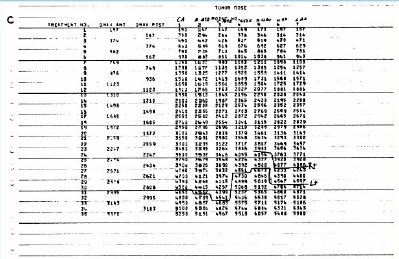
\includegraphics[width=0.6\textwidth]{Imagens/dadoscalc2d.JPG}
            }%
            \caption{Dados de dose diária calculados por um algoritmo 2D para campos irregulares.}
            \label{fig:dadoscalc2d}
        \end{figure}

    \subsection{Campos Assimétricos}

        Os atuais aceleradores possuem jaws colimadores assimétricos, ou seja, cada jaw colimador pode se mover independentemente, diferente dos primeiros sistemas de colimação onde os pares de jaws X ou Y se moviam simetricamente, de modo que a posição de cada jaw com relação ao seu oposto (por exemplo $X_1$ e $X_2$) eram equidistantes do isocentro. 

        É necessário levar em consideração as mudanças no fator de espalhamento do colimador, fator de espalhamento no phantom e na qualidade do feixe off-axis nos dos campos assimetricamente colimados.  A qualidade do feixe off-axis é afetada devido à utilização de filtros aplanadores, utilizados para deixar a dose plana em uma determinada profundidade (normalmente a 10 cm). o filtro aplanador causa um maior endurecimento do feixe na região central do campo quando comparado às periferias do feixe.

        Portanto, para determinar os cálculos considerando campos assimétricos, assume-se que as mudanças na fluência dos fótons espalhados devido à colimação assimétrica é pequena de modo que pode-se assumir que o fator de espalhamento devido à colimação assimétrica é equivalente ao fator de espalhamento causado por uma colimação simétrica que tenha a mesma abertura fornecida pela colimação assimétrica. Essa é uma aproximação razoável a medida que o ponto de cálculo de dose esteja localizado do centro do campo, longe de suas bordas. O espalhamento do phantom também pode ser considerado o mesmo para o campo assimétrico e para um campo simétrico com o mesma dimensão e forma desde que o ponto de cálculo esteja localizado longe das bordas do campo para evitar os efeitos de penumbra. 

        A distribuição de dose devido ao feixe primário varia com a distância lateral a partir do eixo central devido às mudanças na qualidade do feixe lateralmente causadas pelo filtro aplanador. Portanto a PDP, TMR ou TPT ao longo do eixo central para um campo assimétrico não são as mesmas que a de um campo simétrico com mesma forma e tamanho. Além disso, a fluência do feixe em pontos off-axis varia em função da distância a partir do eixo central, possuindo valores diferentes a medida que a distancia varia. Esses efeitos não são enunciados em campos simétricos pois normalmente o alvo é centralizado no campo, e então o alvo e o ponto de cálculo são posicionados ao longo do eixo central da distribuição de dose. Porém, considerando os campos assimétricos, o alvo ou o ponto de interesse pode não estar ao longo do eixo central, e portanto, nesses casos, deve-se fazer uma correção no cálculo da dose, que irá depender da profundidade do ponto e de sua distância a partir do eixo central.

        A planura de um feixe é estabelecida dentro de 80\% do maior tamanho de campo possível na profundidade de 10 cm, tendo uma variação dentro de $\pm$ 3\%; não considerar as correções de dose off-axis para campos assimétricos irá fornecer erros desta magnitude sob essas condições e portando as correções de dose off-axis seguirá as mudanças na planura do feixe em função da profundidade e da distância ao eixo.


        As equações gerais para o cálculo de MU são utilizadas para os cálculos dos campos assimétricos, alterando o fator $OAR(d, x)$ para o fator $POAR(d, x)$. O fator $POAR(d, x)$ é a razão entre a dose em um ponto off-axis devido a radiação primária e a dose no eixo central na mesma profundidade para um campo simétrico amplo. O Fator $POAR(d, x)$ pode ser extraído a partir dos perfis de campo obtidos para o maior campo disponível, em diferentes profundidade, subtraindo componente de espalhamento. Além desse método indireto, existem dois métodos medem diretamente o fator $POAR(d, x)$:

        \begin{enumerate}
            \item Através da medida dos perfis de dose transmitidos através de diferentes espessuras de um absorvedor sob condições de ``boa geometria'' (feixe estreito e grande distância entre o detector e o absorvedor);
            \item Através de um método aproximado que mede os perfis de dose em função da profundidade para um feixe estreito alongado (5 cm x 40 cm). Devido ao perfil de dose do feixe primário ser criado pelo filtro aplanador que possui uma simetria radial, os dados da POAR podem ser tabelados como função da profundidade e da distância radial com respeito ao eixo central.
        \end{enumerate}
    
    \begin{tcolorbox}[width=\textwidth, colback={white}, title={$\bigstar$ \LobsterTwo{Pontos Chave}$\bigstar $}, coltitle={CarnationPink}, colframe={DarkTurquoise}, fonttitle=\LobsterTwo\Large]
    \begin{itemize}[label=\textcolor{CarnationPink}{$\star$}]
        \item Os fatores TAR e BSF são aplicáveis para feixes de baixa energia até a energia do \ce{^{60}Co}, porém eles não podem ser precisamente medidos para feixes de alta energia devido terem medidas realizadas no ar. Nos casos dos feixes de alta energia, são utilizados os fatores TPR ou TMR, onde amos são medidos no tecido. Ambos estes fatores estão relacionados com os fatores de output $S_c$ e $S_p$ que não possuem limitações de energia.
        \item As quantidades dosimétricas utilizadas para a determinação das MU/Dose incluem a PDP, TMR (ou TPR), $S_c$, $S_p$ e os fatores de distância até a fonte em relação ao método de entrega da dose SAD ou SSD com respeito à calibração. Assumindo a $SAD = 100\;cm$, a calibração em termos da SSD, onde a SSD é definida na superfície do phantom sendo igual a 100 cm, a profundidade de calibração definido na profundidade de dose máxima estará em uma distância igual a $100 + d_{max}$ da fonte; Já para a calibração pela SAD a distância da fonte ao ponto de referência na profundidade será exatamente igual à SAD e  a SSD na superfície do phantom será igual a $SAD-d_{max}$ (Assumindo que o fator de calibração é definido na profundidade de dose máxima).
        \item O fator $S_c$ diz respeito ao campo definido pela abertura dos colimadores, normalmente dado pelos valores nominais dos jaws colimadores $x_1, \; x_2, \; y_1\; e\;  y_2$.
        \item O fator $S_p$ diz respeito ao tamanho de campo projetado na profundidade que realmente será utilizado para tratamento, normalmente é dado pelo campo efetivo formado por blindagens realizadas com blocos ou pelo MLC. 
        
        \item A TMR é um caso especial da TPR onde a profundidade de referência é fixada na profundidade de dose máxima ($d_{max}$) que é a mesma para todos os tamanhos de campo para uma determinada energia. Como ao medir $d_{max}$ em função do tamanho de campo, mostra valores diferentes devido ao aumento da contaminação do feixe primário com elétrons em função do aumento do tamanho de campo, a profundidade $d_{max}$ de referência deve ser determinada a partir de uma geometria que minimize a influência da contaminação com os elétrons; ou seja, deve ser definido para o menor campo possível que mantenha as condições de equilíbrio eletrônico (campo \qtyproduct{3 x 3}{cm}).
        
        \item Enquanto a PDP depende da SSD, a TMR e a TPR são praticamente independentes da SSD, dependendo apenas da profundidade do ponto em que se deseja avaliar a dose em relação à superfície. 
        
        \item Os valores da TMR ou da TPR podem ser medidos diretamente em um phantom ou podem ser determinados a partir das medidas da PDP; O mesmo vale para a PDP que pode ser medida diretamente ou ser obtida através dos valores medidos para a TMR ou TPR;
        
        \item Os fatores SMR e SPR representam a componente devido a apenas o espalhamento dos fatores TMR e TPR, ou seja, não consideram a parte da dose no ponto devido ao feixe primário, considerando apenas a dose devido ao feixe espalhado em outro local dentro do campo que alcança o ponto de análise de dose. Esses fatores são úteis para calcular a componente da dose espalhada no ponto devido à geometria de campos irregulares através do método da integral de Clarkson;
        
        \item Para determinar a dose em um ponto off-axis devido a um campo assimétrico, é necessário ter estabelecido o fator $POAR$, também chamado de ``off-center ratio'', que considera a mudança na fluência de energia para alvos que não estão centralizados com o eixo do feixe mas sim, normalmente, centralizados no campo assimétrico que possui fluência de energia variável com a distância lateral definida do eixo à borda do campo que não será simétrica; 
        
    \end{itemize}
    \end{tcolorbox}

\bibliography{ref.bib}
\end{document}
    
        
